\documentclass[letterpaper,11pt]{article}
\oddsidemargin -1.0cm \textwidth 17.5cm

\usepackage[utf8]{inputenc}
\usepackage[activeacute,spanish, es-lcroman]{babel}
\decimalpoint
\usepackage{amsfonts,setspace}
\usepackage{amsmath}
\usepackage{amssymb, amsmath, amsthm}
\usepackage{comment}
\usepackage{float}
\usepackage{amssymb}
\usepackage{dsfont}
\usepackage{anysize}
\usepackage{multicol}
\usepackage{enumerate}
\usepackage{graphicx}
\usepackage[left=1.5cm,top=2cm,right=1.5cm, bottom=1.7cm]{geometry}
\setlength\headheight{1.5em} 
\usepackage{fancyhdr}
\usepackage{multicol}
\usepackage{hyperref}
\usepackage{wrapfig}
\usepackage{subcaption}
\usepackage{siunitx}
\usepackage{cancel}
\usepackage{mdwlist}
\usepackage{svg}
\pagestyle{fancy}
\fancyhf{}
\renewcommand{\labelenumi}{\normalsize\bfseries P\arabic{enumi}.}
\renewcommand{\labelenumii}{\normalsize\bfseries (\alph{enumii})}
\renewcommand{\labelenumiii}{\normalsize\bfseries \roman{enumiii})}


\begin{document}

\fancyhead[L]{\itshape{Facultad de Ciencias F\'isicas y Matem\'aticas}}
\fancyhead[R]{\itshape{Universidad de Chile}}
\rfoot[]{pág. \thepage}

\begin{minipage}{11.5cm}
    \begin{flushleft}
        \hspace*{-0.6cm}\textbf{FI1000 Introducción a la Física Clásica}\\
        \hspace*{-0.6cm}\textbf{Tutor:} Alejandro Cartes
    \end{flushleft}
\end{minipage}

\begin{picture}(2,3)
    \put(366, -10){
\includegraphics[scale=0.9]{2020-1/Imágenes/logo/dfi-fcfm.pdf}}
\end{picture}

\begin{center}
	\LARGE\textbf{Tutoría C2}\\
	\Large{Dinámica - Trabajo y Energía}
\end{center}

\begin{enumerate}\setlength{\itemsep}{0.4cm}

\item 
\begin{enumerate}
    \item Cuatro partículas idénticas de masa $m$ se unen mediante resortes idénticos de masa nula, constante elástica $k$ y longitud natural $L$. El sistema toma la forma de un cuadrado, como se muestra en la figura, mientras rota en torno a su centro con velocidad angular $\omega$. Determine el largo de los resortes.

    \item Una bolita de masa $m$ se encuentra rotando en la superficie de una esfera de radio $R$ con rapidez angular $\omega$. Si la bolita se encuentra atada a una cuerda, como se muestra en la figura, determine cuál es la rapidez angular mínima que la bolita debe tener para que la cuerda no se afloje.
\end{enumerate}

\begin{figure}[H]
    \centering
    \svgpath{../../2021-1/Imagenes/aux9/}
    \begin{subfigure}[t]{0.2\textwidth}
        \centering
        \includesvg[width=1\linewidth]{cuadrao.svg}
        \caption*{Figura (a)}
    \end{subfigure}
    \hspace{8em}
    \begin{subfigure}[t]{0.18\textwidth}
        \centering
        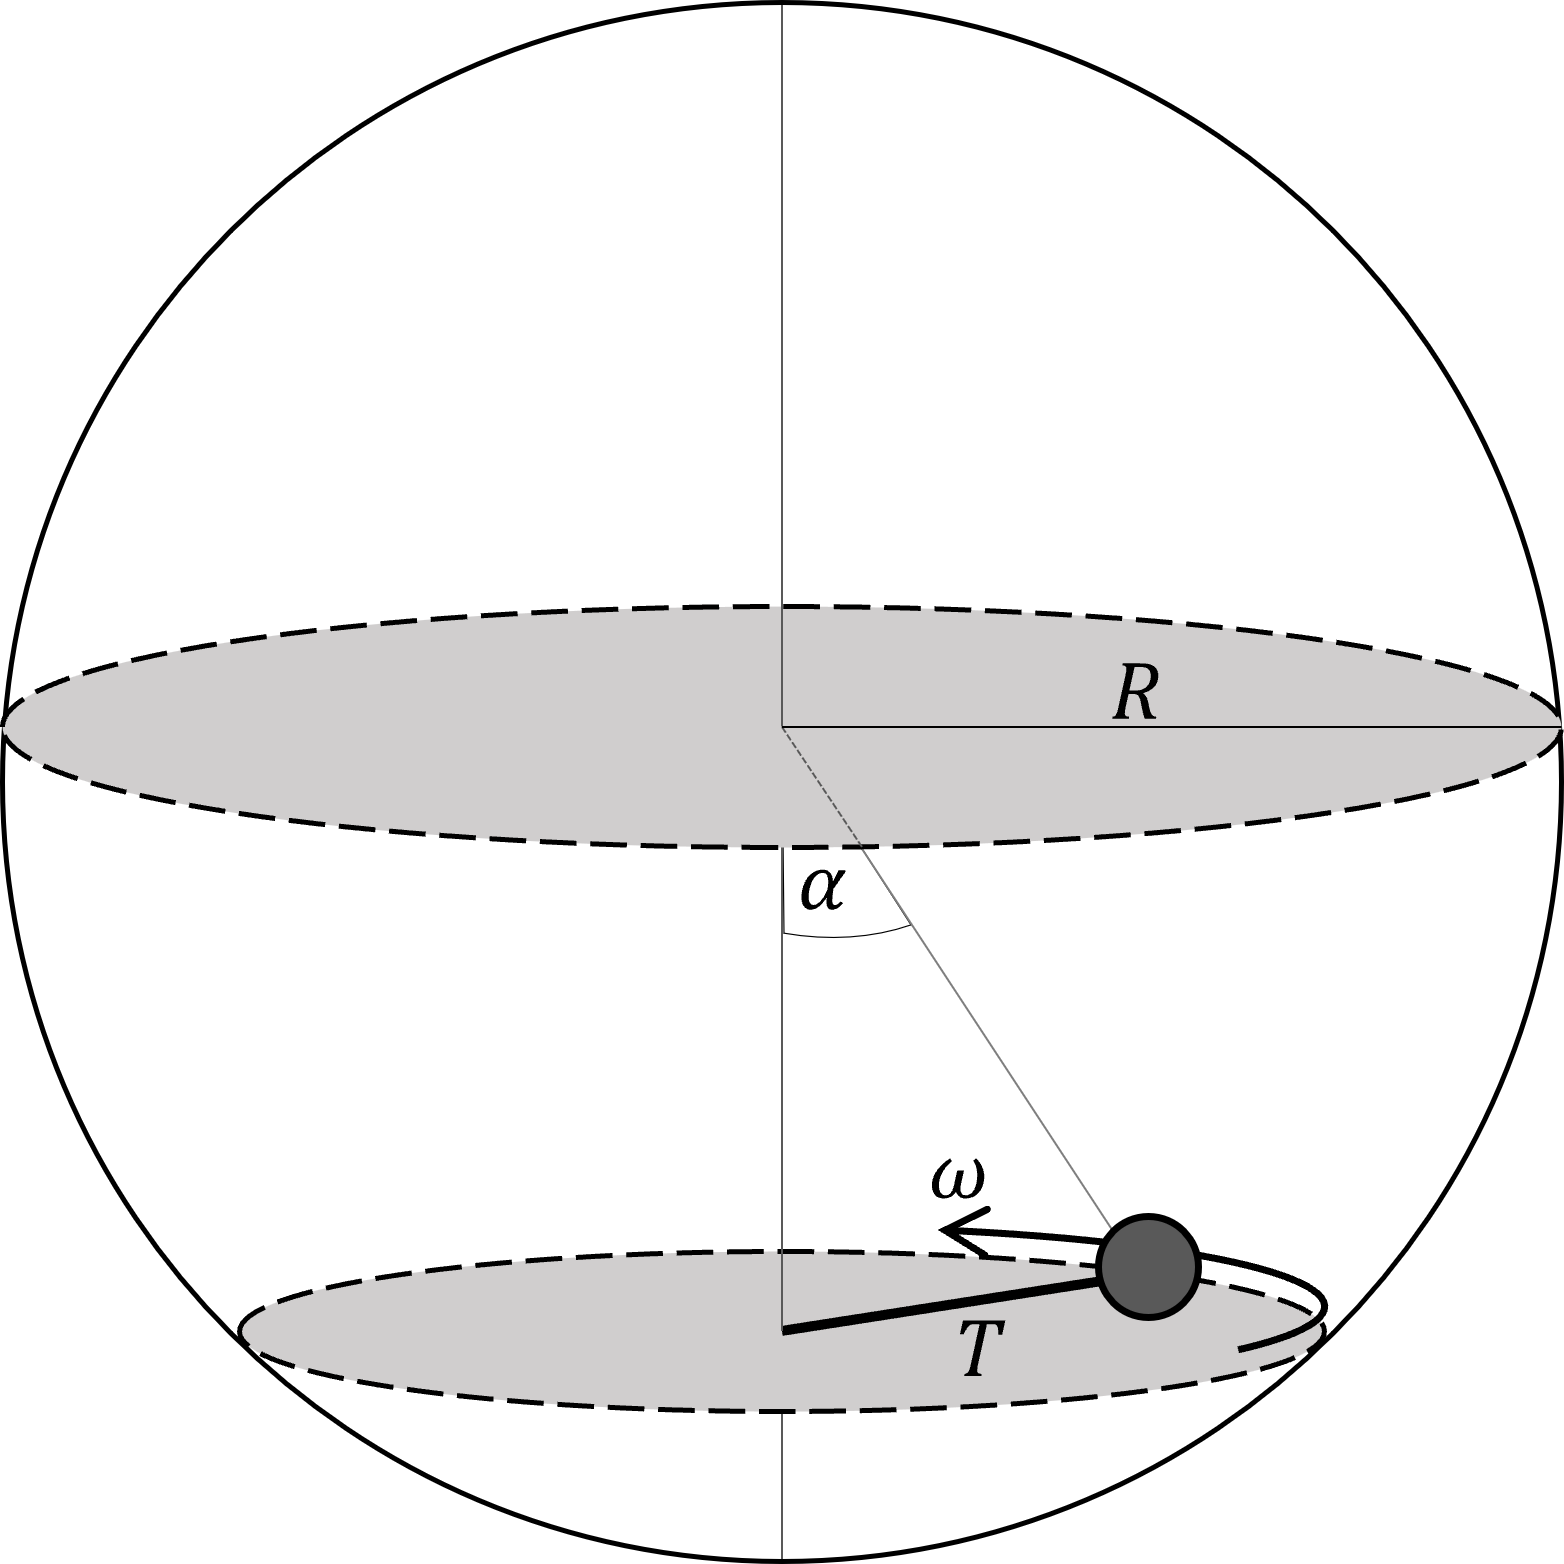
\includegraphics[width=1\linewidth]{2023-1/img/aux_5/esfera.png}
        \caption*{Figura (b)}
    \end{subfigure}
\end{figure}

\item Considere el sistema de la figura. Despreciando el roce, determine la vector aceleración para el bloque de masa $m$ y para la cuña de masa $M$.

\begin{figure}[H]
    \centering
    \includesvg[width=0.24\linewidth]{img/polea.svg}
\end{figure}

% Martes
% \item Un bloque de masa $m$ se desliza por un plano inclinado sin roce de largo $L$ con un ángulo de inclinación~$\theta$ con respecto a la horizontal. Al final de este plano, el bloque se mueve por una superficie áspera con coeficiente de roce cinético $\mu_c$. Determine la distancia $D$ a la cual el bloque se detendrá en esta superficie áspera.

% \begin{figure}[htbp]
%   \centering
%   \svgpath{../../2021-1/Imagenes/ejercicios}
%   \includesvg[width=0.65\linewidth]{ej7.svg}
% \end{figure}

% Miércoles
\item Un bloque de masa $m$ se deja caer por un plano con roce, inclinado en un ángulo $\theta$. Cuando el bloque alcanza el final del plano, se desliza sobre una cinta que se mueve con rapidez $v_b$. Sea $\mu_k$ y $\mu_s$ los coeficientes de roce cinético y estático, respectivamente, de la cinta y del plano inclinado

\begin{minipage}{0.52\linewidth}
    \begin{enumerate}
        \item Determine, en la sección del plano, el trabajo neto
        
        \item Utilizando la parte anterior, determine la rapidez del bloque al llegar al final del plano
        
        \item Determine la distancia $d$ que recorre el bloque a lo largo de la cinta para que alcance la misma rapidez de esta. ¿Qué pasa si la rapidez calculada en la parte (b) es menor? ¿mayor? Separe ambas situaciones
    \end{enumerate}
\end{minipage}
\hfill
\begin{minipage}{0.47\linewidth}
    \begin{figure}[H]
        \centering
        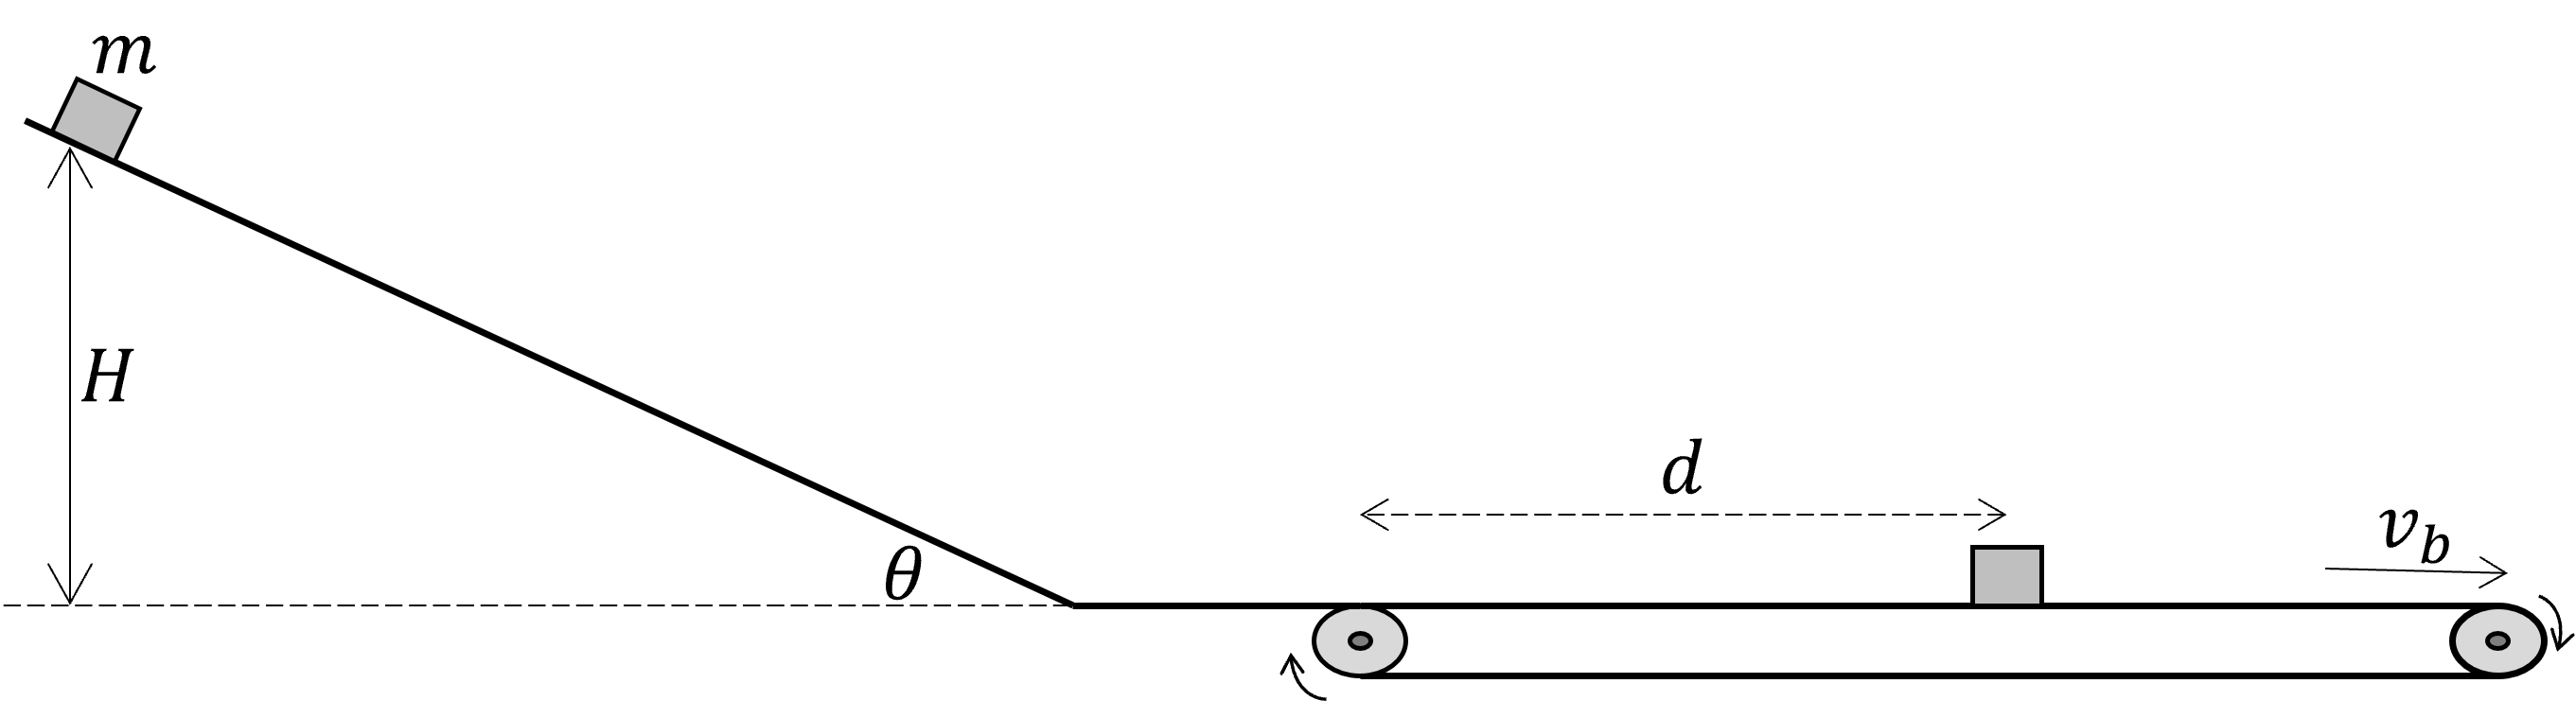
\includegraphics[width=1\linewidth]{2023-1/img/TD 3/cinta.png}
    \end{figure}
\end{minipage}

\item Un bloque de masa $m$ choca con un bloque de masa $M$ en una superficie horizontal con coeficiente de roce cinético $\mu_m$ y $\mu_M$ respectivo a cada masa. Tras la colisión los bloques viajan juntos, pero no pegados, a una rapidez desconocida.
\begin{enumerate}
    \item Si la distancia recorrida por el sistema es $d$, determine la rapidez inicial
    \item El trabajo realizado por $F_{Mm}$ y $F_{mM}$
\end{enumerate}

% Para imágenes vectoriales -> el texto tiene que estar en LaTeX
% \begin{figure}[htbp]
%   \centering
%   \svgpath{../Imagenes/ejercicios}  -> .. irse pa'trás 
%   \includesvg{ej5.svg}
% \end{figure}

\end{enumerate}
\end{document}
